\begin{Problem}
    For each application benchmark, you need to calculate the number of unique 32B instruction and data chunks accessed. Report the instruction and data statistics separately.
    
    In this assignment, we will calculate the memory footprint at a granularity of 32B.

\noindent
    Prepare a table showing the instruction and data footprints of the applications.
\end{Problem}

\begin{Solution}

\begin{figure}[H]
    \centering
    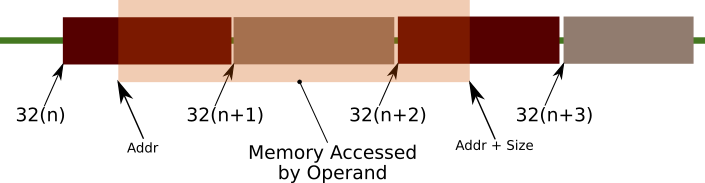
\includegraphics[width=0.9\textwidth]{images/memory_access.png}
    \caption{Schematic representation of Memory access depicting granularity}
    \label{fig:pC:mem_access}
\end{figure}

In the figure \ref{fig:pC:mem_access} all of $32n$, $32(n+1)$ and $32(n+2)$ must be considered for that particular memory access.

Using the above interpretation, we consider memory chunks accessed by the program with respect to both instruction and data memory.
Following are the results:

\begin{table}[H]
    \centering
    \caption{Instruction and Data Memory Chunks accessed}
    \label{tab:pC:chunks}
    \begin{tabular}{| l | c | c |}
        \hline
        \multirow{2}{*}{Application} & \multirow{2}{*}{I. Memory Chunks} & \multirow{2}{*}{D. Memory Chunks} \\
        & & \\
        \hline
        400.perlbench & 2849 & 21106 \\
        \hline
        401.bzip2 & 272 & 317909 \\
        \hline
        403.gcc & 996 & 438547 \\
        \hline
        429.mcf & 64 & 7732611 \\
        \hline
        450.soplex & 625 & 5661102 \\
        \hline
        456.hmmer & 462 & 84599 \\
        \hline
        471.omnetpp & 901 & 529903 \\
        \hline
        483.xalancbmk & 2285 & 595797 \\
        \hline
    \end{tabular}
\end{table}

    
\end{Solution}